\documentclass{protokol}
\leftheader{Určení Planckovy konstanty}
\centerheader{Praktikum IV}
\rightheader{Tomáš Derner}

\begin{document}

  \section*{Úkol}

    \begin{enumerate}
      \item Změřte voltampérové charakteristiky fotonek GKE, GKV.
      \item Rozborem charakteristik zjistěte, která z nich je vakuová a která je plynem plněná.
      \item Změřte VA charakteristiky vakuové fotonky pro záporné hodnoty anodového napětí.
      \item Zpracováním výsledků měření určete hodnotu Planckovy konstanty.
    \end{enumerate}

  \section*{Teorie}

    V tomto praktiku se zabýváme vnějším fotoefektem, při kterém dochází k emisi nositelů náboje z povrchu elektrody osvětlené elektromagnetickým zářením. Fotonka je realizována jako skleněná baňka vyčerpaná na vysoké vakuum nebo naplněná inertním plynem. Na postří\-břeném vnitřním povrchu baňky je nanesena fotokatoda, uvnitř baňky se nachází anoda. 
    
    V případě vakuové fotonky zapojené v propustném směru je voltampérová charakteristika význačná prudkým růstem proudu při zvyšujícím se napětí, po kterém následuje nasycení, při kterém se již proud v závislosti na rostoucím napětí téměř nemění. To je v kontrastu s průběhem VA charakteristiky fotonky plynové, u které je efekt nasycení menší a proud s rostoucím napětím nadále vzrůstá.

    Vakuové fotonky lze využít k určení Planckovy konstanty $h$. Připojíme-li totiž fotonku v záporném směru, budeme nejprve při nulovém napětí pozorovat fotoemisi elektronů s určitou kinetickou energií. Zvyšováním proudu však postupně elektrony musejí překonávat rostoucí potenciál, až při určité kritické hodnotě napětí $V_0$ proud fotonkou ustane. Jelikož kinetická energie elektronů souvisí Einsteinovým vztahem $E = h \nu - A$ s frekvencí dopadajícího záření ($A$ je energie potřebná pro uvolnění elektronu z katody), lze psát závislost kritické hodnoty napětí $V_0$ na frekvenci $\nu$ vztahem 
    \begin{equation} \label{eq:vztah}
      V_0 = \frac{h}{e} \nu + C, 
    \end{equation}
    kde $e$ je náboj elektronu a $C$ je konstanta související s vlastnostmi fotonky. Lineární regresí pomocí tohoto vztahu můžeme tedy získat Planckovu konstantu \cite{pokyny}.

    Protože se ve fotonce při dosažení kritické hodnoty napětí projevuje slabá fotoemise anody, protékající proud není nulový, ale mírně záporný. Je proto nutné hodnotu napětí $V_0$ extrapolovat k hodnotě nasyceného záporného proudu.
    
  \section*{Výsledky}

    \subsection*{Úkol 1 a 2}

      Elektronickým multimetrem se zabudovaným zdrojem napětí jsme proměřili voltampérové charakteristiky fotonek GKE a GKV připojených v propustném směru. Fotonka byla osvě\-tlovaná rtuťovou výbojkou, spektrálním filtrem byla vybrána vlnová délka světla $\lambda = \SI{546}{nm}$. Z grafu na obrázku \ref{fig:u1} je s pomocí popisu tvarů charakteristik v teorii zřejmé, že fotonka GKE je plněna plynem, zatímco GKV je vakuová. Kvůli velkému množství bodů závislosti bylo praktické zobrazit závislosti lomenou čarou propojující tyto body.

      \begin{figure}[H]
        \centering
        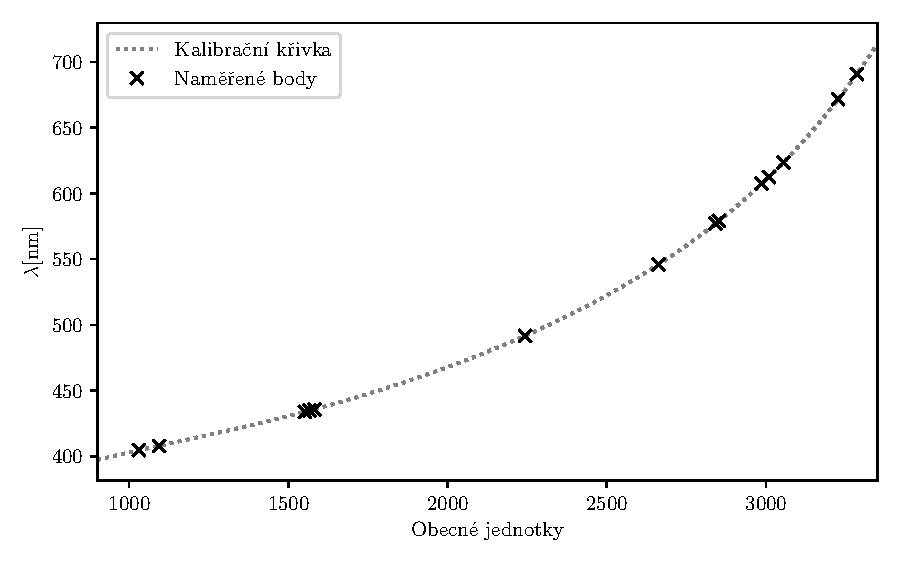
\includegraphics[]{u1}
        \caption{Voltampérové charakteristiky dvou fotonek}
        \label{fig:u1}
      \end{figure}

    \subsection*{Úkol 3 a 4}

      Následně jsme pro 5 vlnových délek dopadajícího světla změřili VA charakteristiky vakuové fotonky v závěrném směru. Rozsah proměřovaných napětí byl volen tak, aby se průnik závislosti s osou $I = 0$ nacházel zhruba v polovině měřeného intervalu a bylo tak dostatek prostoru pro odečtení nasyceného záporného napětí. 

      Extrapolace hodnoty kritického napětí $V_0$ byla provedena lineárním fitem části závislosti. Za hodnotu $V_0$ byla vzata hodnota napětí, při které tato fitová přímka (v grafech červěně) protíná vodorovnou přímku značící hodnotu nasyceného záporného proudu (v grafech šedě). Pro lineární fit bylo vždy vzato posledních pět bodů kladného proudu (to odpovídá intervalu napětí $\SI{0.2}{V}$).

      Naměřené závislosti i s fitovými přímkami použitými k extrapolaci jsou znázorněny v grafech na obrázcích \ref{fig:u3_365} až \ref{fig:u3_578}.

      \begin{figure}[H]
        \centering
        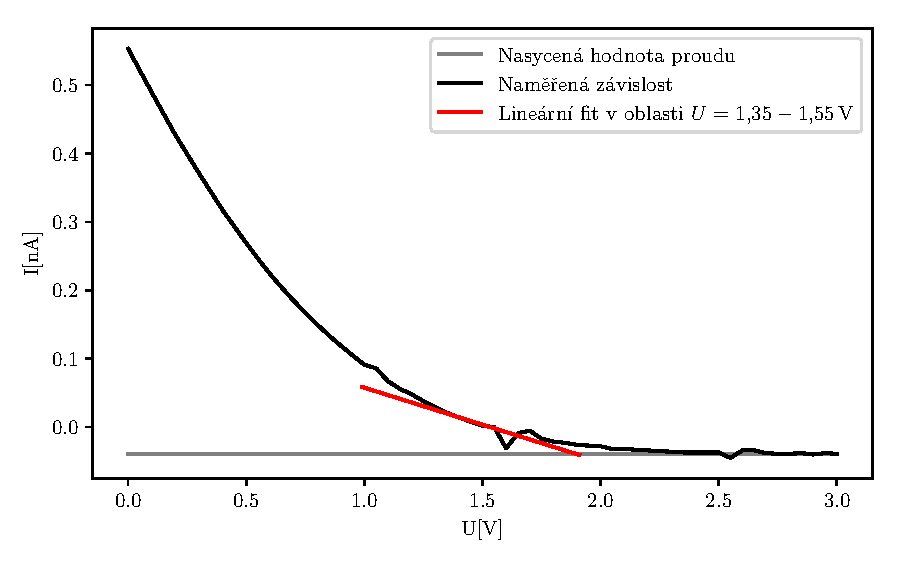
\includegraphics[]{u3_365}
        \caption{Voltampérová charakteristika vakuové fotonky při $\lambda = \SI{365}{nm}$}
        \label{fig:u3_365}
      \end{figure}

      \begin{figure}[H]
        \centering
        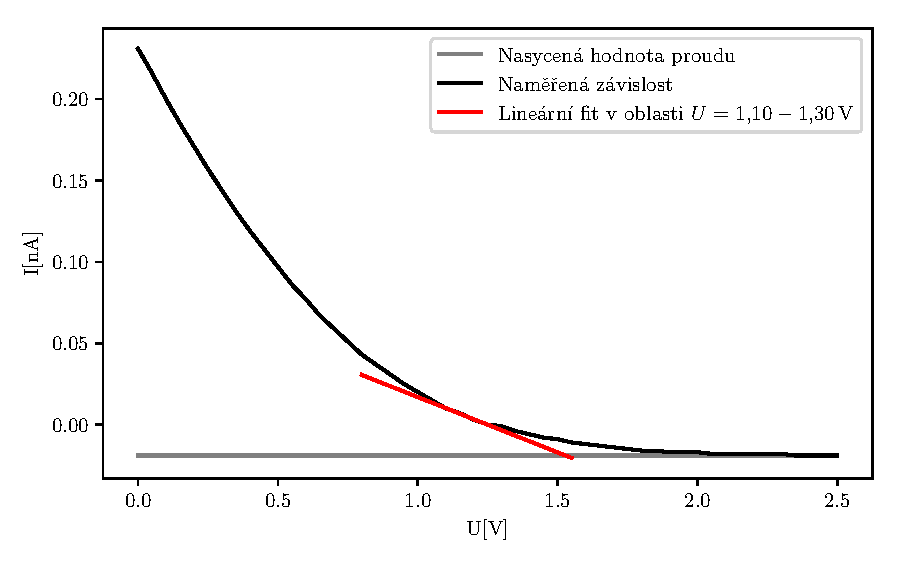
\includegraphics[]{u3_405}
        \caption{Voltampérová charakteristika vakuové fotonky při $\lambda = \SI{405}{nm}$}
        \label{fig:u3_405}
      \end{figure}

      \begin{figure}[H]
        \centering
        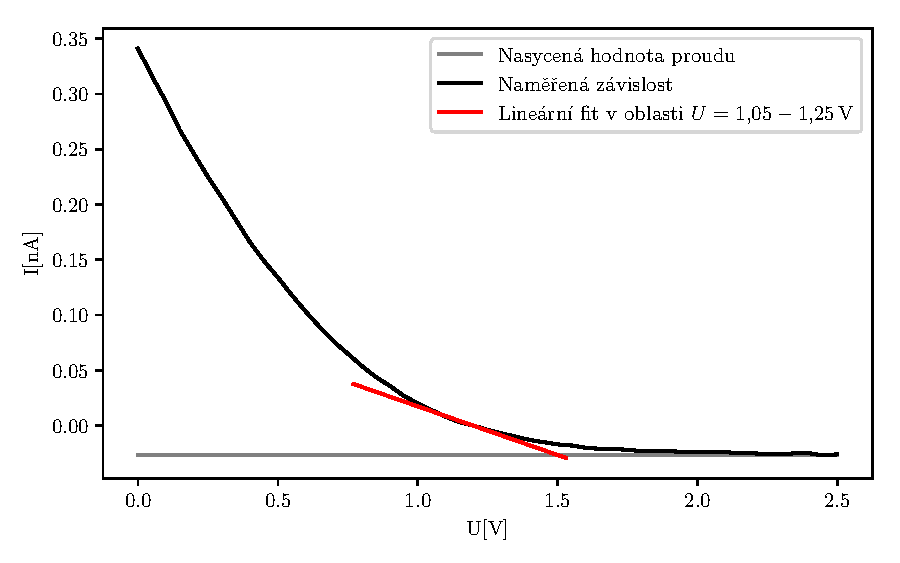
\includegraphics[]{u3_436}
        \caption{Voltampérová charakteristika vakuové fotonky při $\lambda = \SI{436}{nm}$}
        \label{fig:u3_436}
      \end{figure}

      \begin{figure}[H]
        \centering
        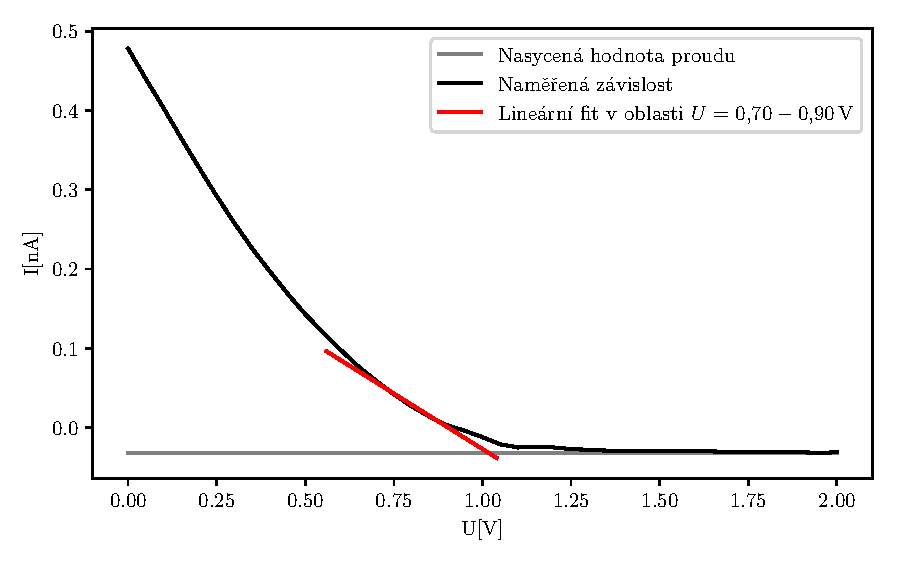
\includegraphics[]{u3_546}
        \caption{Voltampérová charakteristika vakuové fotonky při $\lambda = \SI{546}{nm}$}
        \label{fig:u3_546}
      \end{figure}

      \begin{figure}[H]
        \centering
        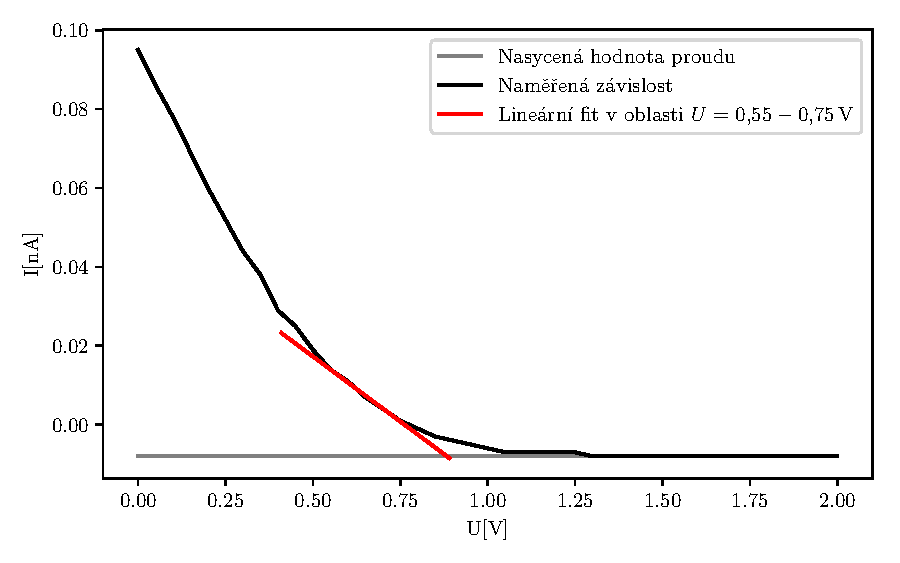
\includegraphics[]{u3_578}
        \caption{Voltampérová charakteristika vakuové fotonky při $\lambda = \SI{578}{nm}$}
        \label{fig:u3_578}
      \end{figure}

    Z grafů byly odečteny hodnoty kritických napětí $V_0$
    $$ V_0^{\SI{365}{nm}} = \SI{1.89 \pm 0.1}{V}, $$
    $$ V_0^{\SI{405}{nm}} = \SI{1.53 \pm 0.1}{V}, $$
    $$ V_0^{\SI{436}{nm}} = \SI{1.50 \pm 0.1}{V}, $$
    $$ V_0^{\SI{546}{nm}} = \SI{1.02 \pm 0.1}{V}, $$
    $$ V_0^{\SI{578}{nm}} = \SI{0.88 \pm 0.1}{V}. $$

    Po přepočtení vlnových délek na frekvence podle vztahu $\nu = \frac{c}{\lambda}$, kde $c$ je rychlost světla, byla v grafu \ref{fig:planck} vynesena závislost kritického napětí $V_0$ na frekvenci dopadajícího záření $\nu$ podle vztahu \eqref{eq:vztah}. Lineárním fitem byla určena hodnota
    $$ \frac{h}{e} = \SI{3.19 \pm 0.24 e-15}{\joule\second\per\coulomb}.$$
    Vynásobením této hodnoty nábojem elektronu získáme hodnotu Planckovy konstanty 
    $$ h = \SI{5.10 \pm 0.56 e-34}{\joule\second}. $$

    Chyba hodnot vlnových délek potažmo frekvencí byla zanedbána, jelikož je zastíněna chybou určení hodnoty $V_0$.

    \begin{figure}[H]
      \centering
      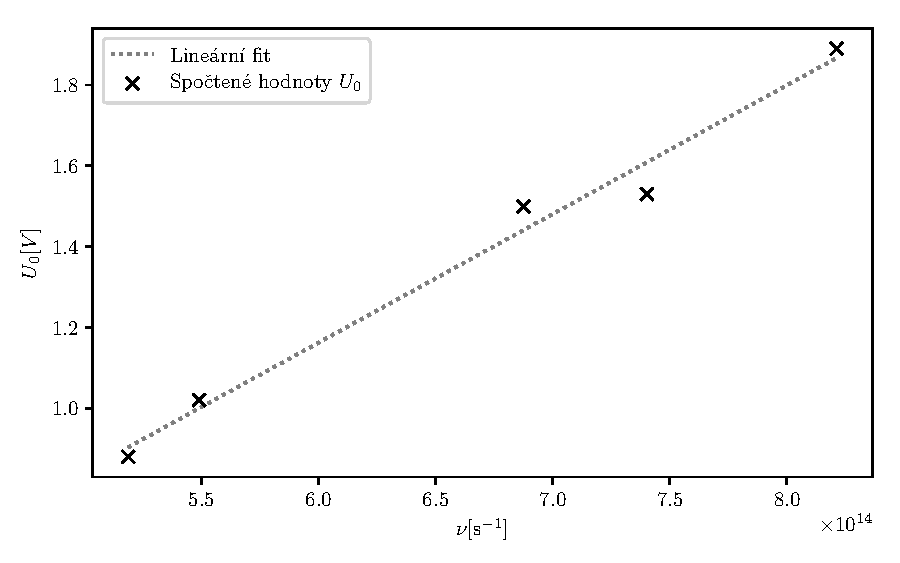
\includegraphics[]{planck}
      \caption{Závislost kritické hodnoty napětí na frekvenci záření podle \eqref{eq:vztah}}
      \label{fig:planck} 
    \end{figure}


  \section*{Diskuse}

    Voltampérové charakteristiky naměřené v úkolu 1 odpovídají teoretickým předpovědím.

    Spočtená hodnota Planckovy konstanty se neshoduje v rámci chyby s tabulkovou hodnotou. To je způsobeno nejspíše větší systematickou chybou určení hodnoty $V_0$. Měření mohlo být také zkresleno nedokonalým seřízením aparatury. Clonka, korigující intenzitu světla dopadajícího na fotonku, totiž nebyla ideálně dovřená.

  \section*{Závěr}

    Z naměřených voltampérových charakteristik fotonek v propustném směru, které se shodují s teoretickou předpovědí, bylo určeno, že fotonka GKE je plynová, fotonka GKV vakuová.

    Pomocí změřených voltampérových charakteristik vakuové fotonky v závěrném směru s různými hodnotami vlnových délek dopadajícího záření byla určena hodnota Planckovy konstanty  
    $$ h = \SI{5.10 \pm 0.56 e-34}{\joule\second}. $$

  \begin{thebibliography}{} 
 
    \bibitem{pokyny}
    Studijní text k měření ``Studium fotoelektrického jevu, určení Planckovy konstanty'', dostupné z\\ \url{https://physics.mff.cuni.cz/vyuka/zfp/zadani/texty/txt_a09}, 9.\,10.\,2018
   
  \end{thebibliography}

\end{document} 